\chapter[Introdução]{Introdução}

\section{Proposta de Implementação}

Ao analisar a história de mixers e equipamentos e o mercado atual, chega-se a conclusão de que a evolução dos equipamentos foi e é realizada partindo de um modelo que se baseia na mixagem feita em vinil. Ao longo do tempo, acrescentou-se novas funcionalidades e formas de interações, porém, na maioria das vezes, mantendo o jogger para atraso e avanço da música, fadder para volume e knobs para frequências.
\par
Além disso, conforme a evolução da microeletrônica, equipamentos começaram a migrar aos poucos para a eletrônica digital, culminando na utilização de um DSP para o processamento do sinal de áudio para comportar formatos de música com baixa compressão como WAV. e FLAC. 
\par
Assim, o que se vê hoje são dois extremos: equipamentos extremamente caros mas que não necessitam da presença de um computador e equipamentos dependentes, que são mais baratos e acabam possuindo melhor qualidade nos processamentos, que dificultam a mobilidade.
\par
Dessa forma, o intuito é conceber um mixer dotado de uma interface inovadora, que se destaque em relação aos modelos tradicionais por sua intuitividade. Para tanto, opta-se pela utilização da Raspberry Pi, aproveitando sua capacidade de processamento de sinais e sua flexibilidade para criar uma interface personalizada. Tal abordagem se mostra vantajosa em comparação com os equipamentos convencionais, como as CDJs, não apenas devido à sua funcionalidade aprimorada, mas também por apresentar um custo mais acessível.

\subsection{Documentação}
Nas seções subjacentes, há uma série de documentações que visam a descrever e delinear o projeto a partir de diferentes óticas. Além disso, a informação contida de forma textual se encontrará melhor descrita graficamente através de diagrama, fluxogramas e outras ferramentas.

\subsection{Levantamento de Requisitos}
\textbf{Requisitos Funcionais:}
\begin{enumerate}[label=\textbullet]
\item O sistema deve permitir ao DJ ajustar o volume de cada canal de áudio individualmente.
\item O sistema deve fornecer controles de equalização (graves, médios, agudos) para cada canal de áudio.
\item O sistema deve permitir ao DJ utilizar tanto CDJs quanto toca-discos.
\item O sistema deve permitir ao DJ escutar canais não ativados ao público (cue).

\end{enumerate}

\textbf{Requisitos Não Funcionais:}
\begin{enumerate}[label=\textbullet]
\item O sistema deve ser capaz de responder aos comandos do DJ com latência mínima, garantindo uma experiência de mixagem fluida.
\item A interface do usuário do sistema deve ser intuitiva e fácil de usar, permitindo que o DJ faça ajustes rapidamente durante a performance.
\item O sistema deve ser confiável e estável, capaz de lidar com longos períodos de uso contínuo sem falhas.
\item O sistema deve oferecer uma qualidade de som de alta fidelidade, garantindo que o áudio reproduzido seja claro e sem distorções.
\end{enumerate}

\textbf{Requisitos de Interface do Usuário:}
\begin{enumerate}[label=\textbullet]
%\item A interface do mixer deve incluir botões físicos ou controles táteis para ajustar o volume, equalização e efeitos de áudio.
\item A interface do mixer deve incluir indicadores visuais, como LEDs ou telas LCD, para mostrar o status dos diferentes canais e configurações.
\item  A interface do mixer deve ser configurável para facilitar a forma de mixagem do DJ.
%\item A interface do mixer deve ser organizada de forma lógica e intuitiva, com controles agrupados por função para facilitar a navegação.
\end{enumerate}

\textbf{Requisitos de Sistema:}
\begin{enumerate}[label=\textbullet]
\item O sistema deve ser compatível com uma variedade de dispositivos de áudio externos, como CDJs e toca-discos.
\item O sistema deve ser alimentado por uma fonte de energia padrão, como uma tomada elétrica.
\item O sistema deve incluir interfaces de entrada e saída de áudio padrão, como conectores RCA ou XLR, para facilitar a conexão com outros equipamentos de áudio.
\end{enumerate}

\textbf{Requisitos de Desempenho:}
\begin{enumerate}[label=\textbullet]
\item O sistema deve ser capaz de lidar com até dois canais de áudio simultaneamente, sem comprometer a qualidade do som ou a responsividade dos controles.
\item O sistema deve suportar uma ampla gama de frequências de áudio, garantindo que os graves sejam reproduzidos com punch e os agudos sejam nítidos e claros.
\end{enumerate}

\textbf{Requisitos de Interface de Usuário:}
\begin{enumerate}[label=\textbullet]
%\item O sistema deve fornecer feedback visual claro para indicar quando um efeito está ativo ou desativado.
\item O sistema deve permitir ao DJ personalizar a aparência e layout da interface do usuário para atender às suas preferências individuais.
\item O sistema deve ser compatível com dispositivos de entrada externos, como controladores MIDI ou dispositivos de toque, para permitir diferentes estilos de interação do usuário.
\end{enumerate}

\textbf{Requisitos de Segurança:}
\begin{enumerate}[label=\textbullet]
\item O sistema deve ser projetado para minimizar o risco de danos aos equipamentos de áudio conectados, como proteção contra sobrecarga ou curto-circuito.
\end{enumerate}

\textbf{Requisitos de Manutenção:}
\begin{enumerate}[label=\textbullet]
\item O sistema deve ser projetado para facilitar a manutenção e reparo, com acesso fácil aos componentes internos e documentação clara sobre procedimentos de serviço.
\end{enumerate}

\textbf{Requisitos de Compatibilidade:}
\begin{enumerate}[label=\textbullet]
\item O sistema deve ser compatível com uma variedade de formatos de áudio comuns, como WAV, MP3 e FLAC.
\end{enumerate}

\subsection{Análise do Questionário}

Um questionário foi aplicado pelo Digital DJ Tips; um portal de notícias e de cursos cuja abrangência possibilitou a coleta de mais de 1500 respostas ao redor do mundo, durante o dezembro de 2023 e janeiro de 2024. O questionário abrangeu informações divididas em seções como: informações demográficas, tipos e experiências, setup (hardware e software), estilos musicais e fontes musicais e, como último, social media. Através da análise do questionário, foi possível levantar algumas histórias de usuários. 

\subsection{Informações Demográficas}
Nesse quesito, obteve-se uma distribuição crescente conforme a idade dos DJs. 25 a 34 anos teve 18,86\%, 35 a 44 teve 28,45\% e 45 a 54 obteve 32,33\%. No questionário, não obteve-se respostas significativas de brasileiros. Dessa forma, esse perfil não corresponderia ao perfil do brasileiro.
\par
Quanto a renda anual em atividades gerais, em dólares, as maiores faixas foram 25k - 50k, 50k - 75k, seguidos por 0 - 15k. Além disso, quanto a renda advindo da atividade de DJ, 40,86\% não recebe pela atividade, já para 34,47\% dos entrevistados 10\% de sua renda advém de discotecagem.

\subsection{Tipo de DJ e Experiência}
A maioria, 53,92\%, havia começado a tocar há mais de 10 anos. Além disso, percebe-se há um aumento de de DJs que permanecem na atividade até 3 anos, porém, depois começa a cair. Porém, percebe-se que a maior faixa é daqueles que permanecem há muito tempo na atividade, há mais de 10 anos.
\par
Outro ponto importante é o tipo de DJ que os entrevistadores são. A maioria, 27,49\% toca regularmente em público, já 25,66\% toca de vez em quando, logo em seguida estão: pessoas que tocam ocasionalmente para amigos e família.
\par
Outro dado importante é que a maioria dos entrevistados são hobbistas/bedroom ou DJs focados em eventos como casamentos, aniversário, corporativos. Em seguida, encontram-se os que chegam a tocar mas não levam a atividade como fonte de renda. Em seguida, encontram-se os que têm a discotecagem como profissão, como: residentes, djs e produtores. Portanto, a maioria são hobbistas e DJs focados em eventos, sem ser clubes.
\par
Porém, um dado interessante é que a maioria deseja se tornar um dj que vive em tour ou que possui residência em algum clube. Além disso, quanto a transmitir os sets, apenas 10\% disnponibiliza online os seus sets produzidos. Porém, quase 50\% almeja a transmissão de seus sets pela internet.
\par
Dessa forma, percebe-se todo tipo de estilo de DJ: aqueles que tocam em locais profissionais que provavelmente já contam com os equipamentos profissionais próprios e conforme cai a porcentagem dos resultados, percebe-se a diminuição da complexidade do equipamento devido ao sistema de som local.

\subsection{Setup - Hardware e Software}
Quanto ao equipamento utilizado, 56\% toca através de um notebook e de uma controladora. Em seguida, 15\% possui XDJ (All-in-one standalone). Além disso, 56\% utiliza Pioneer como marca principal em seus equipamentos, seguido pela Denon. 
\par
Quanto ao montante investido no setup, a maioria gastor entre USD 1500 a 3000, seguidos por USD 1000 a 1500 e USD 3000 a 5000.
\par
Outro dado importante, é que 63\% das pessoas visam realizar uma atualização do setup a cada ano. Dentre aqueles que não podem, metade desses não fazem devido aos custos relacionados. E mesmo entre esses, 53\% gostaria de adquirir Pioneer. 
\par
37\% dos entrevistados disse que, quando são contratados, devem levar o próprio equipamento.
\par
Quanto à inovação mais interessante, segundo os entrevistados, está a possibilidade, que tem sido vista em controladoras atuais, de separar uma música em elementos e ter a capacidade de tanto separar quanto de aplicar efeitos apenas nesse grupo de elementos em tempo real. Além disso, a possibilidade de utilizar uma biblioteca na nuvem e o desenvolvimento de softwares que mixam automaticamente também deixaram os entrevistadores animados. 
\par
Quanto às características mais importantes ao se adquirir novos equipamentos, a qualidade e durabilidade se encontraram em primeiro lugar, seguido de recursos, preços, marcas e integrações.
\par
O software utilizado pelo DJ precisa poder ser integrado ao sistema de mixagem. O software é como a biblioteca é organizada e como o pendrive é organizado. Dessa forma, ao escolher um software, a pessoa deve levar em consideração os equipamentos que ela pode utilizar. Assim, 2/3 dos entrevistados se dividiram entre Rekordbox e Serato DJ.

\subsection{Estilos musicais e aquisição de músicas}

56\% dos DJs mixa utilizando diversos tipos de gêneros. Em contrapartida, 1/4 dos DJs só mixa focado em um estilo. A diferença entre a mixagem entre um estilo e vários é a habilidade de elencar elementos semelhantes ou contrastantes para realizar uma mixagem.
\par
Dentre os gêneros mais tocados, encontram-se house, hip hop, pop, tech house, techno, bass, EDM, disco, deep house e outros. Para servir como base da mixagem, DJs utilizam outros gêneros para servir como construção e presença de elementos. Os gêneros mais utilizados para essa presença são house, disco, hiphop, tech house, deep house, funk e techno. Porém, a presença de gêneros é bem diversa.
\subsection{Proposta de Implementação do Protótipo}

Quais são as funcionalidades necessárias para um Protótipo:

- Volume: o controle de volume exige dois knobs ou sliders: dois knobs ou sliders no total

- Frequência: três knobs para cada canal: 6 no total

- Trim: um knob para cada canal: 2 no total

- Master: 1 knob no total

- Headphone: 1 knob no total

Ao todo, 10 potenciômetros/knobs ou 8 knobs + 2 sliders

Quais botões são necessários?

\begin{itemize}
	\item On/off -> 1 no otal
	\item Cue -> 2 no total
	\item Master -> 2 no
\end{itemize}

\subsection{Diagramas de Subpartes}
\subsection{Diagrama de Integração}
\subsection{Diagrama de Comunicação}
\subsection{Fluxograma}
\subsection{Protótipo de Interface de Usuário}
\subsection{Documento de Especificação Técnica}
\subsection{Documento de Plano de Teste}



\section{Contextualização}

\section{Definição do Problema e Proposta de Pesquisa}
\section{Objetivos}
\subsection{Objetivo Geral}
\subsection{Objetivos Específicos}
\section{\textbf{Estrutura da Monografia}}


\chapter[Fundamentação Teórica e Estado da Arte]{Fundamentação Teórica e Estado da Arte}

Nessa seção, serão abordados conceitos básicos para a compreensão da monografia (teoria, problema e proposta); a começar pela definição de um sinal segundo a literatura,representado por um sinal elétrico, tanto analógico quanto digital; conceituar música e a importância da mixagem realizada por \textit{DJs}, culminando no equipamento utilizado, dando enfoque ao \textit{mixer}, seja na sua história, evolução e no seu estado da arte.


\newpage
\section{Sinal: Conceito}

\begin{citacao}
"Os sinais, que são funções de uma ou mais variáveis independentes, contêm informações sobre o comportamento ou natureza de algum fenômeno, enquanto os sistemas respondem a algum sinal em particular, produzindo outros sinais ou algum comportamento desejado." \cite{oppenheim2010sinais}.
\end{citacao}

Como exemplifica \cite{oppenheim2010sinais}, tensões e correntes ao longo do tempo são funções, ou seja, sinais, enquanto o circuito em si pode ser compreendido como um sistema que reage à entrada aplicada, ao produzir sinais de saída.

Sensores são dispositivos capazes de mensurar grandezas físicas através da captação de sinais elétricos. Dessa forma, a criação desse instrumento permitiu a compreensão de fenômenos físicos. Assim, o monitoramento de grandezas permite que se atue em sistemas físicos a fim de se obter um resultado desejado.
\newline
[O intuito do parágrafo acima é simplesmente realizar uma ponte entre sinais elétricos e quais compreensões um sensor permite que sejam realizadas. De forma que a atuação em um sistema seja realizada a fim de se chegar a um resultado esperado.]

Com o desenvolvimento de sensores na história da instrumentação, foi possível a obtenção da quantização de parâmetros físicos através de sinais elétricos. E dessa forma, a compreensão de fenômenos físicos e, consonante a isso, a construção de sistemas que podem alterar os sinais conforme a resposta desejada. 

\section{Sinal Contínuo}
Dentro das possibilidades do que um sinal pode ser, pode-se classificá-lo como contínuo caso a sua variável independente seja contínua, ou seja, que tenha um valor para cada instante de tempo (variável independente). Por exemplo, entre o intervalo de \textit{t} a \textit{t+1}, há infinitos valores tanto de tempo quanto para o parâmetro em função do tempo, \cite{oppenheim2010sinais}. Um exemplo pode ser o valor de corrente em um resistor alimentado por uma tensão ou um som que gera uma pressão acústica no ar captados pelo sistema auditivo. A Figura \ref{fig01} é um exemplo de um gráfico para um sinal contínuo no tempo. 

\begin{figure}[h]
	\centering
	\includegraphics[scale=0.5]{figuras/fig01.eps}
	\caption{sinal de tempo contínuo}
	\label{fig01}
\end{figure}
\newpage

\subsection{Sinal Discreto}
Em contrapartida a um sinal contínuo em relação a sua variável independente, há outra classificação de sinal denominado de discreto. A sua variável independente é o tempo discreto, que pode ser definido por um conjunto de números inteiros. Caso a variável independente não seja inteira, ou seja, \textit{n} não seja inteiro, não há  valor definido. Dessa forma, entre \textit{n} e \textit{n+1}, não há infinitos valores como há no tempo contínuo. Um exemplo dessa classificação de sinal pode ser . \cite{oppenheim2010sinais}. A Figura \ref{fig02} é um exemplo de um gráfico para um sinal no tempo discreto. 
\newline
[Quando o senhor diz que ao invés de ser um sinal discreto, é um discretizado, o senhor se refere ao exemplo da variação semanal da bolsa de valores. Ou ao conceito explicado na seção?]


\begin{figure}[h]
	\centering
    \includegraphics[scale=0.5]{figuras/fig02.eps}
	\caption{sinal de tempo discreto}
	\label{fig02}
\end{figure}

\subsection{Transformada de Fourier}
Uma ferramenta matemática crucial para a análise de sinais na frequência é a transformada de Fourier, que realiza uma modificação do termo independente, saindo do tempo ou espaço e indo para frequências, também denominada de equação de análise, que pode ser visualizada na equação \ref{eq:03}. \par De forma análoga, transformada inversa, ou a também chamada de equação de síntese, realiza o processo inverso, modificando o sinal representado no domínio da frequência para o seu domínio original, segundo \cite{oppenheim2010sinais}, seja tempo ou espaço. A equação da transformada inversa pode ser visualizada na equação \ref{eq:04}

\begin{equation}  \label{eq:03}
X(e^{j\omega})= \sum_{n=-\infty}^{+\infty} x[n]e^{-j\omega n}
\end{equation}

\begin{equation}  \label{eq:04}
x[n]=\frac{1}{2\pi} \int_{2\pi}^{} X(e^{j\omega})e^{j\omega n} \,d\omega
\end{equation}

\subsection{Teorema da Amostragem}
Devido ao desenvolvimento da computação nas últimas décadas e pela conseguinte diminuição de custos de produção e de aquisição de dispositivos capazes de realizar o processamento digital de sinais, tornou-se muito vantajoso a utilização de sinais no tempo discreto, para que possam ser trabalhados digitalmente, e posteriormente, ou não, serem convertidos novamente para o tempo contínuo, sem a perda da informação inicial. 

O processo de obter um sinal discreto a partir de um sinal contínuo é denominado de amostragem, e para que, a partir do sinal amostrado, reconstrua-se o sinal contínuo original, o sinal e o processo de amostragem devem preencher alguns requisitos.

Para que um sinal seja amostrado, é necessário que o intervalo de amostragem, ou seja, o espaçamento entre duas amostras seja regular. A cada período $T$, uma amostra é adquirida, resultando em uma frequência de amostragem $f = 1/T$.
Ao passar essa função do domínio do tempo para o domínio da frequência, obter-se-á uma banda de frequências que compõe o sinal no domínio do tempo.

\begin{figure}[h]
	\centering
    \includegraphics[scale=0.5]{figuras/fig03.eps}
	\caption{espectro do sinal amostrado com Ws > 2Wm}
	\label{fig03}
\end{figure}

Ao observar a Figura \ref{fig03}, sendo a componente $\omega_M$ a maior frequência angular presente no sinal do tempo, $\omega_s$ a frequência de amostragem, constata-se que $\omega_M<(\omega_s-\omega_M)$ segundo Oppenheim e Willsky \cite{oppenheim2010sinais}. Dessa forma, $\omega_s>2\omega_M$. Caso a frequência de amostragem seja menor que $\omega_M$, haverá sobreposição das bandas adjacentes, e, por conseguinte, a reconstrução do sinal não será possível. Ao respeitar esse requisito, o sinal pode ser recuperado ao utilizar um filtro passa-baixas de com a frequência de corte maior que $\omega_M$ e menor que $\omega_M-\omega_s$.
Essa análise é o Teorema de Amostragem que infere que a:

\begin{equation} \label{eq:01}
\omega_s>2\omega_M
\end{equation}

em que

\begin{equation} \label{eq:02}
\omega_s=\frac{2\pi}{T}
\end{equation}

O parâmetro $\omega_M$, que deve ser menor que metade da frequência de amostragem  $\omega_s$, recebe o nome de frequência de Nyquist \cite{oppenheim2010sinais}.
\par
Esse teorema foi explicitado na literatura por Shannon \cite{Shannon} mas foi apontado anteriormente por Nyquist \cite{nyquist} [EXPLICAR DIREITO O QUE A FRASE A SEGUIR SIGNIFICA]. A partir dela, compreende-se a suficiência da representação de um sinal pela série de Fourier por 2TW amostras, no qual T é a duração de uma função e W é a frequência mais alta que compõe o sinal.

\subsection{Aliasing}
Quando a frequência de amostragem não está de acordo com o critério de Nyquist, ou seja, menor que o dobro da frequência mais alta, não se tem a reconstrução do sinal, já que, ao realizar a filtragem passa-baixa, na banda $/omega_M$ haverá componentes da banda adjacente.

\subsection{Teorema da Quantização}

Após a amostragem de sinais, obtém-se um conjunto de sinais. Para que esses sinais, pertencentes ao domínio contínuo, possam ser processados, é necessário que se faça a quantização digitalmente. A quantização é um processo no qual se determina intervalos de valores, atribuindo cada valor amostrado a um valor quantizado em função do intervalo no qual o valor se insere. Para cada sinal amostrado, é atribuido um valor quantizado.

\begin{figure}[h]
	\centering
    \includegraphics[scale=0.4]{figuras/fig04.eps}
	\caption{quantização de amplitudes em tempo discreto}
	\label{fig04}
\end{figure}

Para que determine com precisão os valores dos intervalos da quantização, o maior e o menor valor obtido pós amostragem são os limites dos valores de amplitudes discretos. Na Figura \ref{fig04}, observa-se o processo a partir do qual, para cada valor obtido na amostragem, há um intervalo correspondente que passará a representar esse sinal. \par O intervalo de amplitude discreta da Figura \ref{fig04} varia de -32768 a +32767, totalizando 65536 possíveis amplitudes discretas, ou seja, $2^{16}$ possíveis amplitudes. Dessa forma, cada amplitude pode ser representada por uma palavra binária de 16 bits. A quantidade de bits a ser utilizada determinará a quantidade de intervalos possíveis, o que, por conseguinte, determinará a precisão da quantização, devido a um erro gerado.\par Cada processo de quantização deve levar em conta a precisão necessária e os limites do intervalo de valores possíveis. Ao final, o procedimento de quantização é essencial para as conversões AD (analógico para digital).

A quantização, o processo de digitalizar a amplitude, é descrita pelo Teorema de Quantização de Widrow \cite{widrow}, segundo  Zölzer \cite{zolzer2008digital}.

\subsection{Reconstrução do Sinal}
A transformação do sinal do tempo discreto para o tempo contínuo, em diversas aplicações, é necessário após algum processamento de sinal realizado segundo Oppenheim e Willsky \cite{oppenheim2010sinais}.
\par
Para que essa reconstrução aconteça, é necessário que o sinal tenha a banda limitada e que se tenha sido utilizada a frequência de amostragem adequada. Uma forma mais simples de implementar a interpolação, segundo Oppenheim e Willsky \cite{oppenheim2010sinais}, é o retentor de ordem zero, que mantém o sinal no mesmo nível até que chegue a próxima amostra, a partir da qual, o nível se alterará para a amplitude desta nova amostra.
\par
Há ordens maiores para os retentores, e, segundo Oppenheim e Willsky \cite{oppenheim2010sinais}, a própria interpolação linear, às vezes, é denominada de retentor de primeira ordem. Um fato a que se deve se atentar é que a reconstrução garante a igualdade entre os valores do sinal inicial e do reconstruído para aqueles instantes em que ocorreram as amostragem.  Conforme a necessidade, pode-se aumentar a ordem do retentor.
\par
Na Figura \ref{fig05}, há o retentor de ordem zero, que mantém o nível da última amostra por um período T. Método que pode ser utilizado na reconstrução de um sinal.

\begin{figure}[h]
	\centering
    \includegraphics[scale=0.4]{figuras/fig05.eps}
	\caption{retentor de ordem zero como amostragem ou reconstrução de um sinal}
	\label{fig05}
\end{figure}

Já na Figura \ref{fig06}, há a interpolação linear para a reconstrução de um sinal. A linha pontilhada é o sinal original e a linha contínua é o sinal reconstruído. 

\begin{figure}[h]
	\centering
    \includegraphics[scale=0.4]{figuras/fig06.eps}
	\caption{interpolação linear entre amostras}
	\label{fig06}
\end{figure}


\section{Som e Música}
Nesta seção, será apresentada uma abordagem histórica, conceitual e técnica entre a natureza do som e a mixagem realizada por um \textit{DJ}. A partir do som, a música será definida e grandezas físicas serão abordadas. Posteriormente, serão abordados cenários históricos e técnicos acerca do início de gravações musicais e da discotecagem. Em seguida, com um enfoque mais atual, será exposto um contexto contemporâneo acerca da mixagem realizada a partir de um \textit{DJ}; que realiza uma seleção musical em função de características de cada música; que realiza transições a fim de se criar uma experiência musical única.

\subsection{Conceito físico}
Segundo Moyses \cite{moyses}: "... corpos em vibração produzem sons ...". Dessa forma, é necessário que haja um meio para que esse som se propague. Esse meio pode ser líquido, viscoso, sólido ou gasoso (como a atmosfera). De acordo com o mesmo autor, "... ondas sonoras na atmosfera são ondas longitudinais, associadas a variações de pressão, ou seja, compressões e rarefações ...". \par Dessa forma, a oscilação de um objeto, ao provoca constantemente compressão e rarefação, altera a densidade na camada adjacente ao meio pelo qual o som será transmitido, gerando uma diferença de pressão que causará um deslocamento adjacente. Portanto, o ciclo de propagação de um som pode ser visualizado na Figura \ref{fig07}.

\begin{figure}[h]
	\centering
    \includegraphics[scale=0.7]{figuras/fig07.eps}
	\caption{ciclo de propagação do som}
	\label{fig07}
\end{figure}

Conforme indica Moyses \cite{moyses}, há parâmetros quantitativos que vão influenciar na percepção auditiva: intensidade, altura e timbre. A intensidade se relaciona com a amplitude da onda sonora. A altura se relaciona com a banda na qual aquele som está localizado, seja nas frequências baixas, tendo uma característica grave, seja aguda, tendo sua banda localizada em altas frequências em relação à banda de frequência audível pelo ouvido humano. Já o timbre são sons que possuem a mesma frequência principal, que o autor chama de "tom fundamental da frequência", porém, possuem outras componentes em frequências maiores, que tornam o som reconhecível, apesar de terem o mesmo tom fundamental da frequência.

\subsection{Audição Humana}
Como Farnell observa \cite{farnell}, apesar que o corpo humano possa sentir vibrações de 1 a 20Hz, o ouvido humano é capaz de produzir a sensação de som a partir de 20 Hz até 10 kHz ou 20 kHz, dependendo da idade do ouvinte. A banda normal na qual a voz humana se localizada fica entre 300 e 3000 Hz, porém, harmônicos advindos de sons reais superam esse limite, inclusive superando os 20 kHz.
Dessa forma, ao utilizar o Teorema de Amostragem, presumi-se que a taxa de amostragem mínima, para que a reconstrução de um som amostrado seja realizada perfeitamente, seja de no mínimo 40 kHz. 

\subsection{História da Gravação e Reprodução de Som}
A partir do som, a humanidade foi capaz de criar uma expressão artística denominada música, que cria a possibilidade da expressão de ideias, sentimentos, identificações, culturas e formas de entretenimento. Além disso, devido a evolução da tecnologia no século XX proporcionou uma grande difusão da música devido às novas possibilidades da gravação e reprodução. 
\par
O primórdio da gravação de um som é atribuído ao Thomas Edison, conforme Roads \cite{roads1996computer}, ao inventar o fonógrafo em 1877. Ao longo da história, aperfeiçoou-se a forma de gravação, armazenamento e reprodução de música, seguido por gramofone, gravadores de fios, fita magnética, vinil. Esses dispositivos utilizavam gravação analógica.
\par
O primeiro formato digital amplamente utilizado foi o CD. Outros formatos digitais tentaram alcançar a mesma popularidade do CD, como o MiniDisc, DVD de áudio e o Blu-Ray áudio; porém, somente os arquivos digitais, destaque ao MPEG-2 Audio Layer III, mais conhecido como MP3, conseguiram alcançar e superar a popularidade do CD. A esse sucesso se deve a utilização de métodos eficientes de compressão e de compartilhamento, que possibilitou o padrão como o principal meio de compartilhamento de música, acompanhando a ampliação do acesso ao computador e de dispositivos digitais capazes de reproduzir música se tornaram acessíveis.

\subsection{Disc Jockeys \textit{DJs}}
Cada novo formato de mídia possibilitou novas formas de circulação de música. Cada mudança de formato de mídia provocou uma transformação na forma como a música é apreciada, partindo de apresentações ao vivo, passando reproduções via rádio, culminando em reproduções em qualquer lugar que houvesse um aparelho capaz de reproduzir a mídia. Com isso, surgiram pessoas que eram especializadas em realizar curadoria de músicas, o que influenciou muito e modificou o consumo de música, e transmitiam as músicas advindas de vinis.
\par
Houve uma grande luta, segundo apontado por Brewster e Broughton \cite{lastnight}, para que DJs, que estavam transmitindo sua seleção nas rádios, pudessem ter apoio de gravadoras, porém, após a Segunda Guerra, a Capital Records formalizou esse apoio após perceber o potencial de divulgação de DJs em rádios. Esse sucesso que era localizado, pois cada \textit{DJ} de uma região tinha influência sobre o que a população de da região na qual a sua rádio tinha alcance, teve a potência de desenvolver gêneros e vertentes novas, uma vez que eles eram criadores de tendência. 
\par
Em 1943, Jimmy Savile, ao ver que um amigo foi capaz de conectar a saída de um gramofone a um rádio valvulado, como saída do sinal de áudio, teve a ideia de realizar um pequeno salão de dança no qual gravações de jazz seriam tocadas enquanto as pessoas poderiam dançar sem que houvesse a presença de uma banda. E assim se deu o início de um clube, segundo Brewster e Broughton \cite{lastnight}. Em seu segundo evento, Jimmy Savile trocou o rádio valvulado por um alto falante. A quantidade de pessoas nesse salão cresceu e Jimmy chegou a implementar essa ideia em inúmeros clubes em toda Inglaterra. Em um projeto específico, para diminuir o tempo de transição entre duas músicas, Jimmy teve a ideia de utilizar dois toca-discos.
\par
Em 1957, conforme Brewster e Broughton \cite{lastnight}, Bob Casey promovia festas em ginásios de escola nas quais utilizava um toca disco conectado a um pequeno alto falante. Utilizando o sistema de áudio do ginásio, posicionava um microfone à saída do alto falante e transmitia em um sistema de áudio ampĺificado o que era tocado nos toca-discos. O seu pai, um engenheiro de som, criou um sistema no qual havia dois toca-discos, em 1955, com controle de volume para permitir a comutação entre os discos e também permiti-lo comentar acerca do disco enquanto o volume da música era abaixado.
\par
De acordo com  Brewster e Broughton \cite{lastnight}, em 1964, durante The World's Fair em Nova Iorque, foi apresentado, por Alex Rosner, primeiro sistema estéreo no qual se utilizou dois canais de áudio, o que representou um grande avanço na experiência de escuta. Inspirados em sistemas de som utilizados na Broadway, David Mancuso e Alex Rosner criaram, para o The Loft (uma famosa festa alternativa), um sistema de som composto por \textit{subwoofer} (alto-falantes dedicados aos tons graves) e \textit{tweeters} (alto-falantes dedicados aos médios).
\par
Já em 1971, Alex Rosner criou o primeiro \textit{mixer} estéreo para \textit{DJ}, visto na Figura \ref{fig08}, o Rosnie, para the Haven Club (um clube famoso da época). Esse equipamento contava com duas saídas: uma para o fone de ouvido e outra para as caixas de som; foi desenvolvido de forma que era possível selecionar de forma independente quais canais estavam ativos no fone, retorno da música para o \textit{DJ}, e quais estavam na saída principal. Além disso, o mesmo controle \textit{on/off} foi implementado para o microfone. 
\begin{figure}[h]
	\centering
    \includegraphics[scale=0.4]{figuras/fig08.eps}
	\caption{Rosnie - inventado por Alex Rosner}
	\label{fig08}
\end{figure}
\par
O Rosnie foi o primeiro \textit{mixer}, para aplicações fora de estúdios, capaz de controlar o ganho de bandas de frequências. Diferente das soluções anteriores que apenas conseguiam controlar o volume dos canais, esse equipamento possibilitou, que de forma natural, mixassem com dois discos simultaneamente, de forma que as transições realizadas fossem extremamente suaves, muitas vezes não compreendendo quando acabava uma música e começava outra. Porém, esse equipamento não foi criado com o intuito comercial.
\par
Louis Bozak, auxiliado por Alex Rosner, criou o CMA-10-2DL em 1971, visto na Figura \ref{fig10}, primeiro mixer estéreo comercializado que instantaneamente se tornou padrão nos clubes da época.

\begin{figure}[h]
	\centering
    \includegraphics[scale=0.6]{figuras/fig10.eps}
	\caption{CMA-10-2DL - Primeiro mixer estéreo comercial}
	\label{fig10}
\end{figure}
\par
Em 1972, a Technics criou o toca-disco SL-1200, Figura \ref{fig14}, que se tornou padrão entre os clubes devido ao \textit{driver} do motor, que proporcionava durabilidade, estabilidade e precisão, o que auxiliava a mudança do BPM, simplificando o \textit{beat matching} (sincronia de batidas) para a sincronia de duas músicas.

\begin{figure}[h]
	\centering
    \includegraphics[scale=0.25]{figuras/fig14.eps}
	\caption{toca-disco SL-1200}
	\label{fig14}
\end{figure}

A partir de uma colaboração entre duas gigantes da indústria da música, Sony e Phillips criaram o CD em 1979, uma nova mídia capaz de armazenar e reproduzir músicas de forma extremamente compacta, leve e mais barata do que o vinil. No ano seguinte, a mesma colaboração desenvolveu o Red Book Audio, o formato de arquivo que viria a ser utilizado no CD, que utiliza PCM (\textit{Pulse Code Modulation}) na sua codificação. Esses desenvolvimentos culminaram em 1982 no início do consumo de CDs, que popularizou ainda mais o consumo de música ao redor do mundo.

Em 1986, a empresa Rane criou um mixer, Figura \ref{fig15}, focado para \textit{DJs} cuja qualidade aproximava-se bastante àquelas praticadas em estúdios de música, MP 24 DJ Club Mixer, o que possibilitou um aumento na qualidade do som reproduzido em clubes.
\begin{figure}[h]
	\centering
    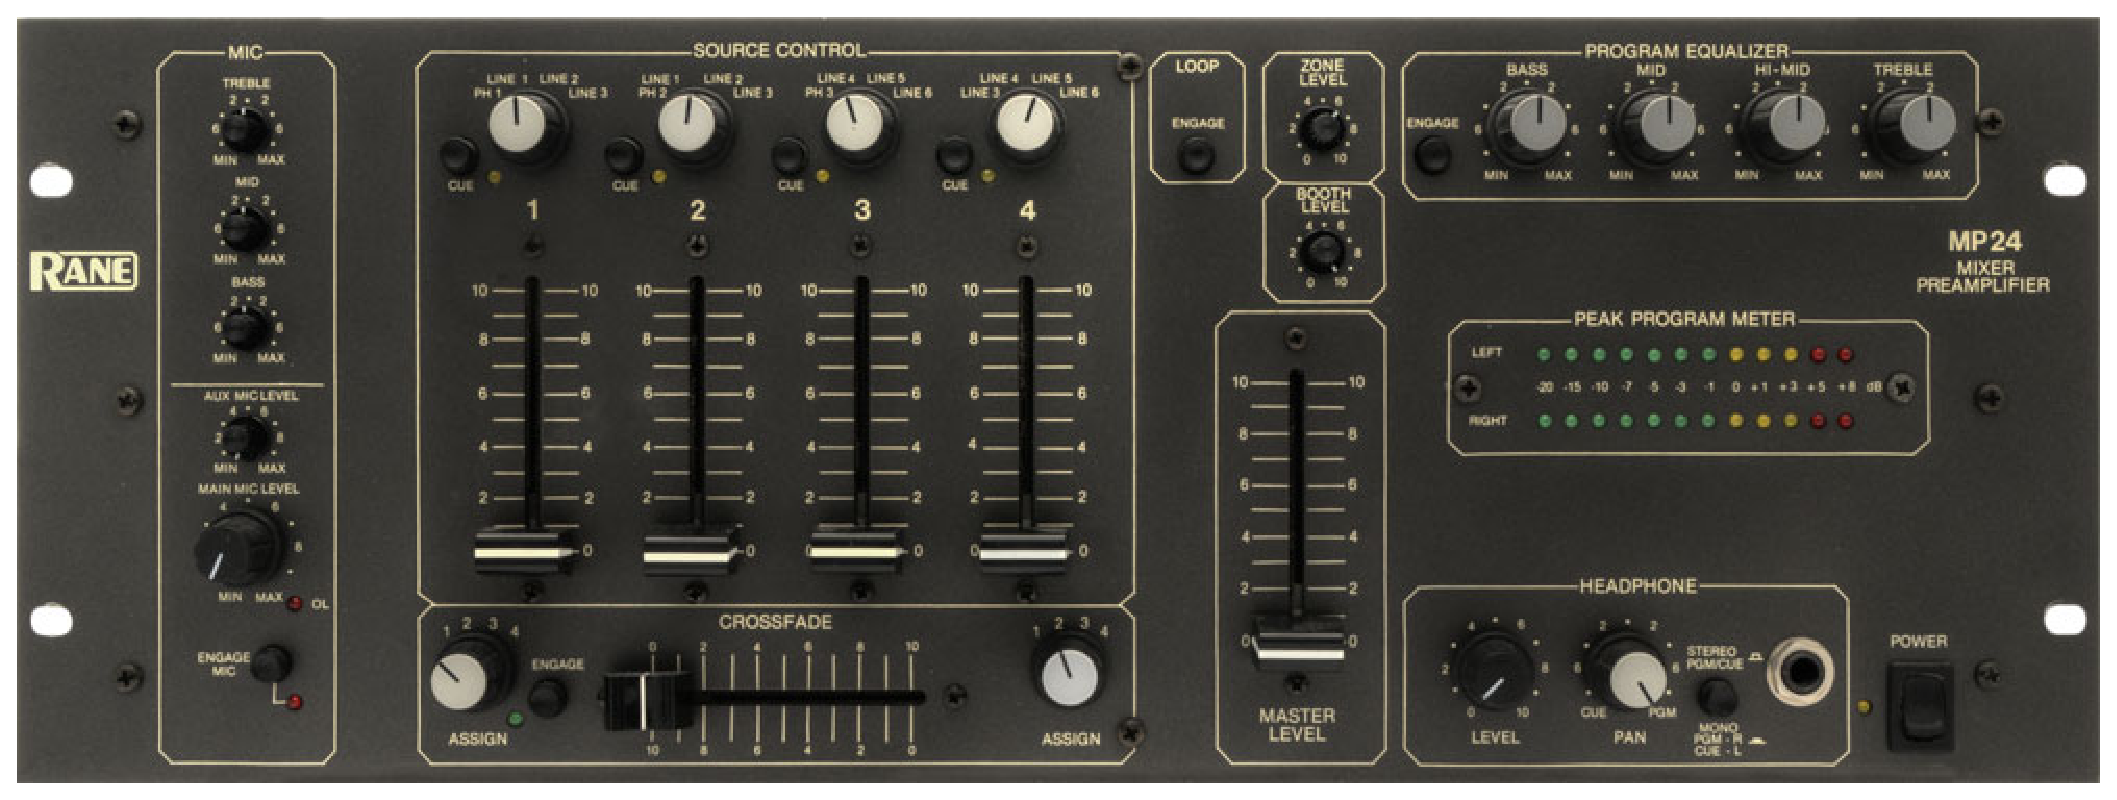
\includegraphics[scale=0.3]{figuras/fig15.eps}
	\caption{mixer criado pela Rane}
	\label{fig15}
\end{figure}

\par
Em 1991, segundo  Brewster e Broughton \cite{lastnight}, criou-se o MP3, um formato de permitiu a compressão do arquivo de áudio de forma que eliminasse conteúdo redundante. Rapidamente, esse método permitiu o compartilhamento massivo de músicas pela internet.


Nos anos 90, uma empresa que viria a ser a gigante dos equipamentos focados em \textit{DJs}, a Pioneer, começou o lançamento de uma série de equipamentos que possibilitou a ampliação e a facilidade da atividade do DJ. Em 1992, a empresa criou a primeira CDJ, um equipamento que unifica inúmeras funções necessárias a mixagem, com suporte para CD. Já em 2001, a empresa lançou uma CDJ com leitor de cartões de memória e em 2007 a mesma lançou uma CDJ capaz de ler dispositivos USB; o que possibilitou que DJs não mais precisassem carregar toda sua discografia consigo, necessitando apenas de um dispositivo de memória digital para ter a sua coleção em mãos.

\begin{figure}[h]
	\centering
    \includegraphics[scale=0.15]{figuras/fig13.eps}
	\caption{CDJ-300 - primeira CDJ da Pioneer}
	\label{fig13}
\end{figure}

\par
Na década de 2010, grandes empresas possibilitaram o \textit{DJ} de tocar músicas que estavam armazenada nas nuvens e músicas que estivessem disponíveis em plataformas de streaming. Em 2024, a Apple lançou o Vision Pro, um óculos de realidade aumentada capaz de emular equipamentos de \textit{DJ}, sendo necessário apenas um óculos de VR para que um \textit{DJ} pudesse demonstrar suas habilidades e sua coleção, advinda de árdua pesquisa. Esse equipamento pode ser visto na Figura \ref{fig16}.

\begin{figure}[h]
	\centering
    \includegraphics[scale=0.3]{figuras/fig16.eps}
	\caption{mixagem virtual com o Apple Vision Pro}
	\label{fig16}
\end{figure}

Ainda que haja muitas soluções inovadoras a respeito de formas de mixagem, a configuração que mais se encontra hoje é formada por duas CDJs e um mixer, conforme a Figura \ref{fig17}.

\begin{figure}[h]
	\centering
    \includegraphics[scale=0.3]{figuras/fig17.png}
	\caption{configuração mais encontrada}
	\label{fig17}
\end{figure}

Porém, há ainda configurações que evocam a qualidade sonora como aspecto primordial. Para esse público, continuam-se produzindo equipamentos analógicos que memoram \textit{layoutes} de \textit{mixers} \textit{vintages}, como os \textit{rotary mixers}, como pode ser visto na Figura \ref{fig18}

\begin{figure}[h]
	\centering
    \includegraphics[scale=0.2]{figuras/fig18.png}
	\caption{\textit{rotary mixer}}
	\label{fig18}
\end{figure}

\par
A mixagem não se limita ao entretenimento em um clube. O papel de um curador de músicas advém do tempo das rádios, e, conforme a tecnologia de reprodução, armazenamento e gravação de música evoluiu, a curadoria musical se tornou mais acessível. 

A mixagem transcende a mera função de entretenimento em uma balada. Desde a expansão do conceito de música feito por John Cage \cite{cage}, no qual música se torna qualquer som, várias expansões conceituais tanto teóricas quanto práticas foram realizadas. Uma mix pode ser tanto o ato de um produtor musical ponderar a presença de cada instrumento ou cada canal em uma música ou o ato de criar uma nova música a partir de várias, com o ato de criar uma colagem sonora. 
\par
Uma mix possui estrutura e enredo, com início, meio e fim. Também diversos propósitos como entretenimento, relaxamento, meditação, cura, dança, apreciação e pesquisa, dentre outros. Além disso, os ambientes de circulação são variados, incluindo páginas de \textit{streaming}, festivais, festas e até mesmo sessões individuais de \textit{bedroom djing} (\textit{DJs} que apenas tocam na sua própria casa, em geral, aprendendo a mixar). Nesse cenário, a liberdade do criador se estende para incluir não apenas misturas de músicas de diferentes gêneros, mas também a incorporação de trechos de áudio de entrevistas, livros, filmes, paisagens sonoras e arte sonora, resultando em uma experiência única.
\par
Além disso, a adição de performances ao vivo, com a utilização de sintetizadores e qualquer dispositivo capaz de gerar som, amplia ainda mais as possibilidades criativas. Desde o uso de sinais elétricos provenientes de eletrodos até a integração de elementos inusitados, como performances ao vivo, as opções são verdadeiramente infinitas, limitadas apenas pela imaginação do criador.

\newpage
\subsection{Parâmetros físicos}
Quando um \textit{DJ} mixa músicas, alguns parâmetros devem ser considerados durante uma música ou no momento da transição entre duas, tais como batidas por minuto (BPM), tom, volume, ganho e presença de componentes em bandas de frequência como graves, médios e agudos.
\par
A evolução dos equipamentos de \textit{DJs} pode ser descrita pelo acréscimo do controle de cada parâmetro citados acima, prezando por um design que facilite tomadas de decisões rápidas com a menor latência possível na saída de áudio, e melhorando também o processamento do áudio de forma que tenha a melhor qualidade possível.
\par
Para a construção de uma melhor atmosfera musical, o controle de bandas de frequência é o mais importante, permitindo a adição e a subtração de elementos de uma música para a criação de uma nova música, que pode ser usado em um momento de transição entre músicas ou para dar uma nova roupagem a uma música. Por exemplo, acrescentar batidas a uma música que não tenha batidas, ou acrescentar vocal a uma música que seja somente instrumental.
\par
O equalizador foi criado, segundo Izhaki \cite{mixing}, pelo Bell Labs com o intuito de ajustar o que era transmitido e o ouvido devido à atenuação de altas frequências durante a transmissão do sinal pelos fios. Porém, para a produção musical, o equalizador é utilizado para manipular o conteúdo de bandas de frequências de diversos elementos musicais. 
Para a produção musical, considera-se sete bandas para a equalização.
\par 
Cada banda representa elementos que possuem características semelhantes. Conforme Izhaki \cite{mixing}, as bandas de frequências de sons audíveis podem ser divididas em:


\begin{itemize}
	\item Subgrave: entre 20 e 60 Hz estão os elementos como bumbo e baixo
	\item Graves baixos: entre 60 e 120 Hz estão tonalidades associadas ao bumbo e ao baixo
	\item Médios graves: entre 120 a 250 Hz onde estão as frequências fundamentais que ditam os tons naturais dos instrumentos
	\item Médios: entre 250 Hz a 2 kHz onde estão harmônicos de baixa ordem de vários instrumentos
	\item Médios Altos: entre 2 e 6 kHz onde há harmônicos complexos
	\item Agudos ou Brilho: entre 9 a 20 kHz onde há pouca energia para muitos instrumentos, porém, ainda assim é uma banda importante por estar associada ao brilho na música.
\end{itemize}

A quantidade de bandas e as definições dos intervalos pode variar entre teóricos, bem como entre equipamentos. Dessa forma, esses intervalos não são a regra. Porém, quando se fala sobre DJs, a maioria dos equipamentos acaba dividindo o espectro de áudio em três bandas: graves, cuja banda varia de 20 a 250 Hz; médios, de 250 Hz a 4 kHz; e agudos, de 4 kHz a 20 kHz.
\par
A essa escolha de bandas reduzidas se deve a necessidade de simplicidade e rapidez no uso, além de que em cada dessas três bandas há elementos semelhantes bastante definidos, que auxiliam muito na construção de uma boa mixagem. A Figura \ref{fig09} ilustra os dois tipos de divisões de bandas apresentados acima. 

\begin{figure}[h]
	\centering
    \includegraphics[scale=0.4]{figuras/fig09.eps}
	\caption{espectro de áudio}
	\label{fig09}
\end{figure}


\subsubsection{Equipamentos}
Os equipamentos utilizados por \textit{DJs} ao longo do tempo evoluíram. Partiram de equipamentos improvisados utilizados para outra finalidade até que foram inventados dispositivos para a finalidade específica foram criados.
Há inúmeras configurações possíveis para se realizar uma mixagem. Primeiramente, deve-se saber qual a fonte de música é utilizada. Caso sejam vinis, deve-se utilizar toca-discos. Caso a fonte seja um dispotivo de memória digital como pendrive ou cartão de memória, no qual há uma série de músicas organizadas por um software de gerenciamento de música, deve-se utilizar uma CDJ. Caso o \textit{DJ} queira fazer performances live na qual ele produz músicas ao vivo, pode-se utilizar notebooks, sintetizadores, samplers ou sequenciadores e inúmeros outros 


%https://daily.redbullmusicacademy.com/2019/06/evolution-of-dj-mixers
%https://www.rane.com/history
%https://medium.com/@soarkxbeta/dj-mixers-series-technology-adapted-to-the-artists-perspective-part-one-90cd4b1f4b27
%https://medium.com/@soarkxbeta/dj-mixers-series-a-technological-invention-turned-to-the-artistic-perspective-part-two-ce6bbbdfb2d4]
% Segundo Laurin Schaffhausen, os mixers clássicos coloriam os sinais, o que não é algo significamente ruim. -> Colocar um parâmetro de distorção do sinal para verificar esse efeito. Coloração pode dar mais vivacidade devido a um ganho em determinada banda. Talvez emular esses brilhos. 
% [Dúvida: qual a diferença entre um vinil analógico e um vinil digital(final dos anos 90)]
% Rotary mixers hoje são produzidos pelas empresas Vestax e Rane
% E&S foi uma empresa criada em colaboração entre um dj Deep e um engenheiro eletrônico. Produzem duas unidades por semana em Paris. 
% Outras empresas no mesmo estilo, pequenas, foram criadas pós E&S, como a Can Electric e Condensa, para ficcionados por Rotary Mixers, principalmente focados em djs que utilizam vinil. 
% Giles Smith produziu o seu próprio mixer - TPI Sound
% Alguns dizem que os Rotary soam melhor do que os com faders mas isso só pode ser dito devido aos componentes eletrônicos serem projetados com a ênfase na qualidade sonora. Tendem a ser estritamente analógicos. 
% O que se sabe é que um controle rotativo acaba sendo mais preciso do que um fader.
% Outra empresa de mixer é a Mastersounds -> Exclusão do EQ de 3 bandas. 
% Os parâmetros para classificar um mixer como bom são muito subjetivos. Pode ser o design, qualidade do áudio, limpeza do som, movimento suave e limpo nos botões, portabilidade, preço, recursos como efeitos. São inúmeros. Além disso, cada pessoa tem seu gosto pessoal. 

% Mixers rotativos têm sido mantidos em um padrão elevado de qualidade de produção. Seus usuários estão amplamente conectados a uma variedade mais caracterizada de mixagem com som orgânico, como disco, música house, Balearic e estilos semelhantes.
%------------------------------------------
%Equipamentos de reprodução -> Revisar a parte de cima e reduzir conforme esses links

% https://medium.com/@soarkxbeta/the-evolution-of-record-players-from-early-beginnings-to-modern-times-part-one-f5f40b39b6e3
% https://medium.com/@soarkxbeta/the-evolution-of-record-players-from-early-beginnings-to-modern-times-part-two-635b8cb8f84d
% https://medium.com/@soarkxbeta/the-evolution-of-record-players-from-early-beginnings-to-modern-times-part-three-77bd2a9c811c
\newpage
\section{Mixer}
% https://medium.com/@soarkxbeta/dj-mixers-series-a-technological-invention-turned-to-the-artistic-perspective-part-two-ce6bbbdfb2d4
Um dispositivo que está sempre em qualquer \textit{layout} montado é o \textit{mixer}, cuja função é a de misturar e controlar canais de entrada de áudio. Quanto ao controle, inúmeras são as possibilidades, mas a mais usual é a de fornecer controle de bandas de frequência para canais de entrada de áudio. Cada dispositivo que reproduz música é lido como um canal de entrada. E esse equipamento é tanto capaz de controlar as bandas de frequência, quanto somar os sinais de áudio, gerando um sinal de saída, que é ligada a alto-falantes. 
\par
Os parâmetros para classificar um \textit{mixer} como bom são muito subjetivos. Podem ser o design do equipamento, qualidade do áudio, distorção do som, manipulação precisa dos botões, ergonomia, portabilidade, preço, recursos como efeitos, referências históricas, integrações com \textit{software} ou outros equipamentos. Além disso, cada pessoa tem seu gosto pessoal e o seu jeito de mixar prezando determinados aspectos.
\par
O desenvolvimento da conexão entre dispositivos de áudio, segundo Winer \cite{winer}, deve considerar três pontos: o sinal de áudio, impedâncias (de entrada e saída) e o tipo de conector.

\subsection{Potência de Sinal de Áudio}

Comumente, encontra-se uma entrada \textit{phono} em \textit{mixers}, correspondente aos dispositivos como toca-discos ou qualquer outro que emita sinais na ordem de miliVolts. Esses sinais necessitam de uma amplificação realizada posteriormente por um amplificador de potência para serem processados pelo sistema do \textit{mixer}. Alguns dispositivos possuem a tensão de saída tão baixa que necessitam de um pré-amplificador para que o sinal possa estar na faixa ideal para que sua potência seja amplificada, para que esteja em um nível de linha.
\par
Outra entrada comumente encontrada é a \textit{line}, que são sinais que já estão em nível de linha. Conforme Winer \cite{winer}, esses sinais possuem dois níveis padrões que são -10 dBV, em equipamentos não balanceados, e +4 dBu, para equipamentos balanceados. Equipamentos de linha profissional costumam a ser balanceados, ou seja, tensões RMS em torno de 1,23 V. Enquanto equipamentos não balanceados são de consumo, por exemplo, aparelhos de som, reprodutores de música e TVs, tensões em torno de 0,316 V.
% [INSERIR TABELA DE CONVERSÃO DE NÍVEIS DE SINAIS EM V, dBV e dBu]

\subsection{Cabeamento}

Condutores desbalanceados apresentam um fio para transmitir o sinal e possuem um terra em comum para gerar a referência \cite{bartlett}. Na Figura \ref{fig12}, é possível verificar a transmissão através de cabos desbalanceados de um sinal acrescido de um ruído.

\begin{figure}[h]
	\centering
    \includegraphics[scale=0.4]{figuras/fig11.eps}
	\caption{fio desbalanceado}
	\label{fig12}
\end{figure}

Já condutores balanceados são cabos que utilizam dois condutores para transmitir o sinal, cobertos por uma blindagem. Ao final da transmissão, os sinais passam por um diferenciador capaz de extrair boa parte dos ruídos adquiridos nos fios durante a transmissão \cite{bartlett}. Um esquemático dos fios para condutores balanceados se encontra na Figura \ref{fig11}.

\begin{figure}[h]
	\centering
    \includegraphics[scale=0.4]{figuras/fig12.eps}
	\caption{Fio Balanceado}
	\label{fig11}
\end{figure}

\subsection{Conectores de 1/4”, 1/8” (3,5 mm) e 2,5 mm}

Para realizar a comunicação entre dispositivos, é necessário que haja tanto a transmissão de sinais elétricos quanto conectores. Cada tipo de conector possui vantagens relacionadas à transmissão de sinais, seja por: quantidade de canais, distância, potência, blindagem e interferência.

Um dos conectores mais conhecidos é o $1/4"$ , Figura \ref{fig19}, principalmente utilizado em instrumentos como guitarras, violões, teclados e outros, podem ser encontrados em amplificadores e mixers, ou seja, em geral para o transporte de níveis baixos de potência. Devido à sua construção física que conta com dois condutores de sinais e um terra, esse tipo de conector pode ser aplicado em sinais estéreos não balanceados ou sinais mono balanceados \cite{bartlett}.

\begin{figure}[h]
	\centering
    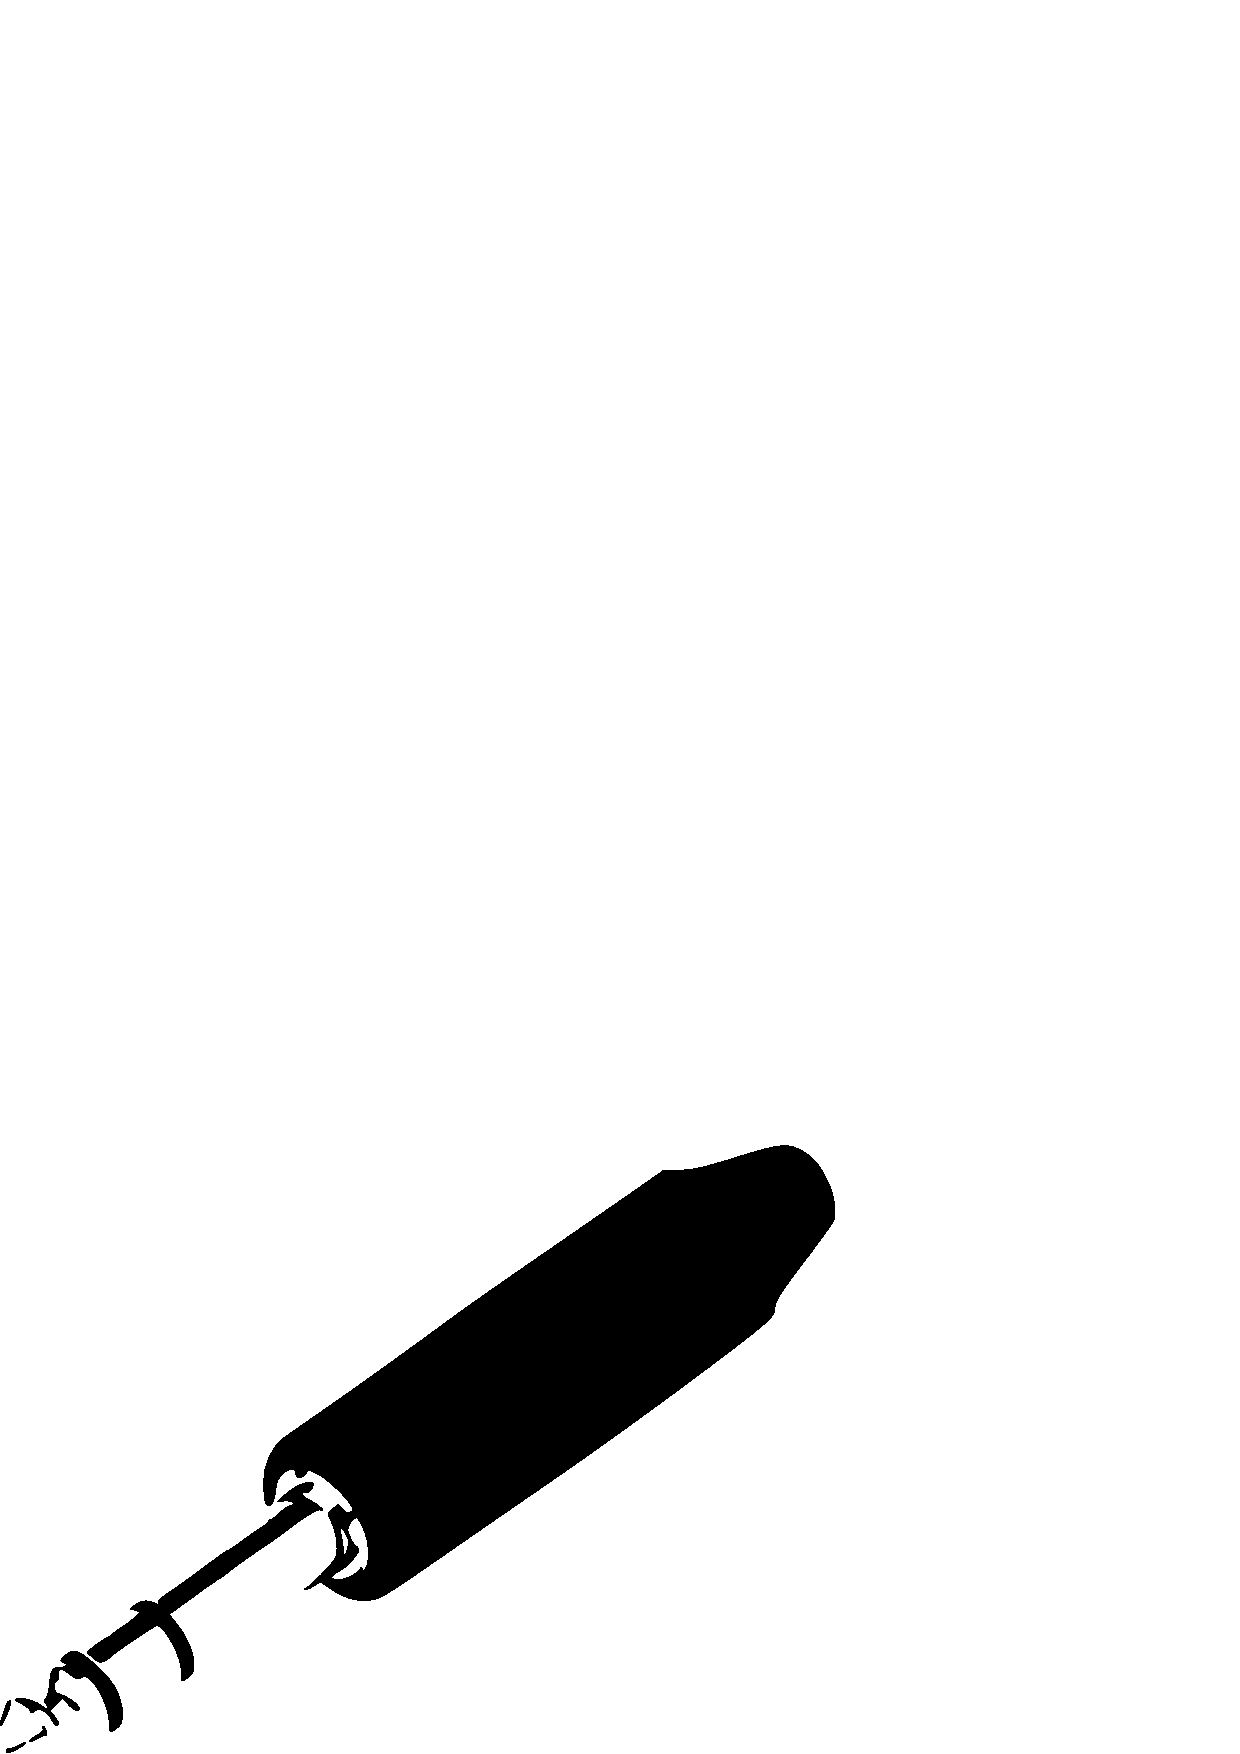
\includegraphics[scale=0.2]{figuras/fig19.png}
	\caption{plug 1/4$"$}
	\label{fig19}
\end{figure}

Existe uma versão menor da versão 1/4", sendo o 1/8", Figura \ref{fig20}, ou mais conhecido como 3.5 mm. Esse tipo de conector é muito encontrado em celulares, dispositivos de reprodução de música e alto-falantes. Internamente, ele possui a mesma construção do 1/4" e também consegue transmitir os mesmos tipos de sinais.

\begin{figure}[h]
	\centering
    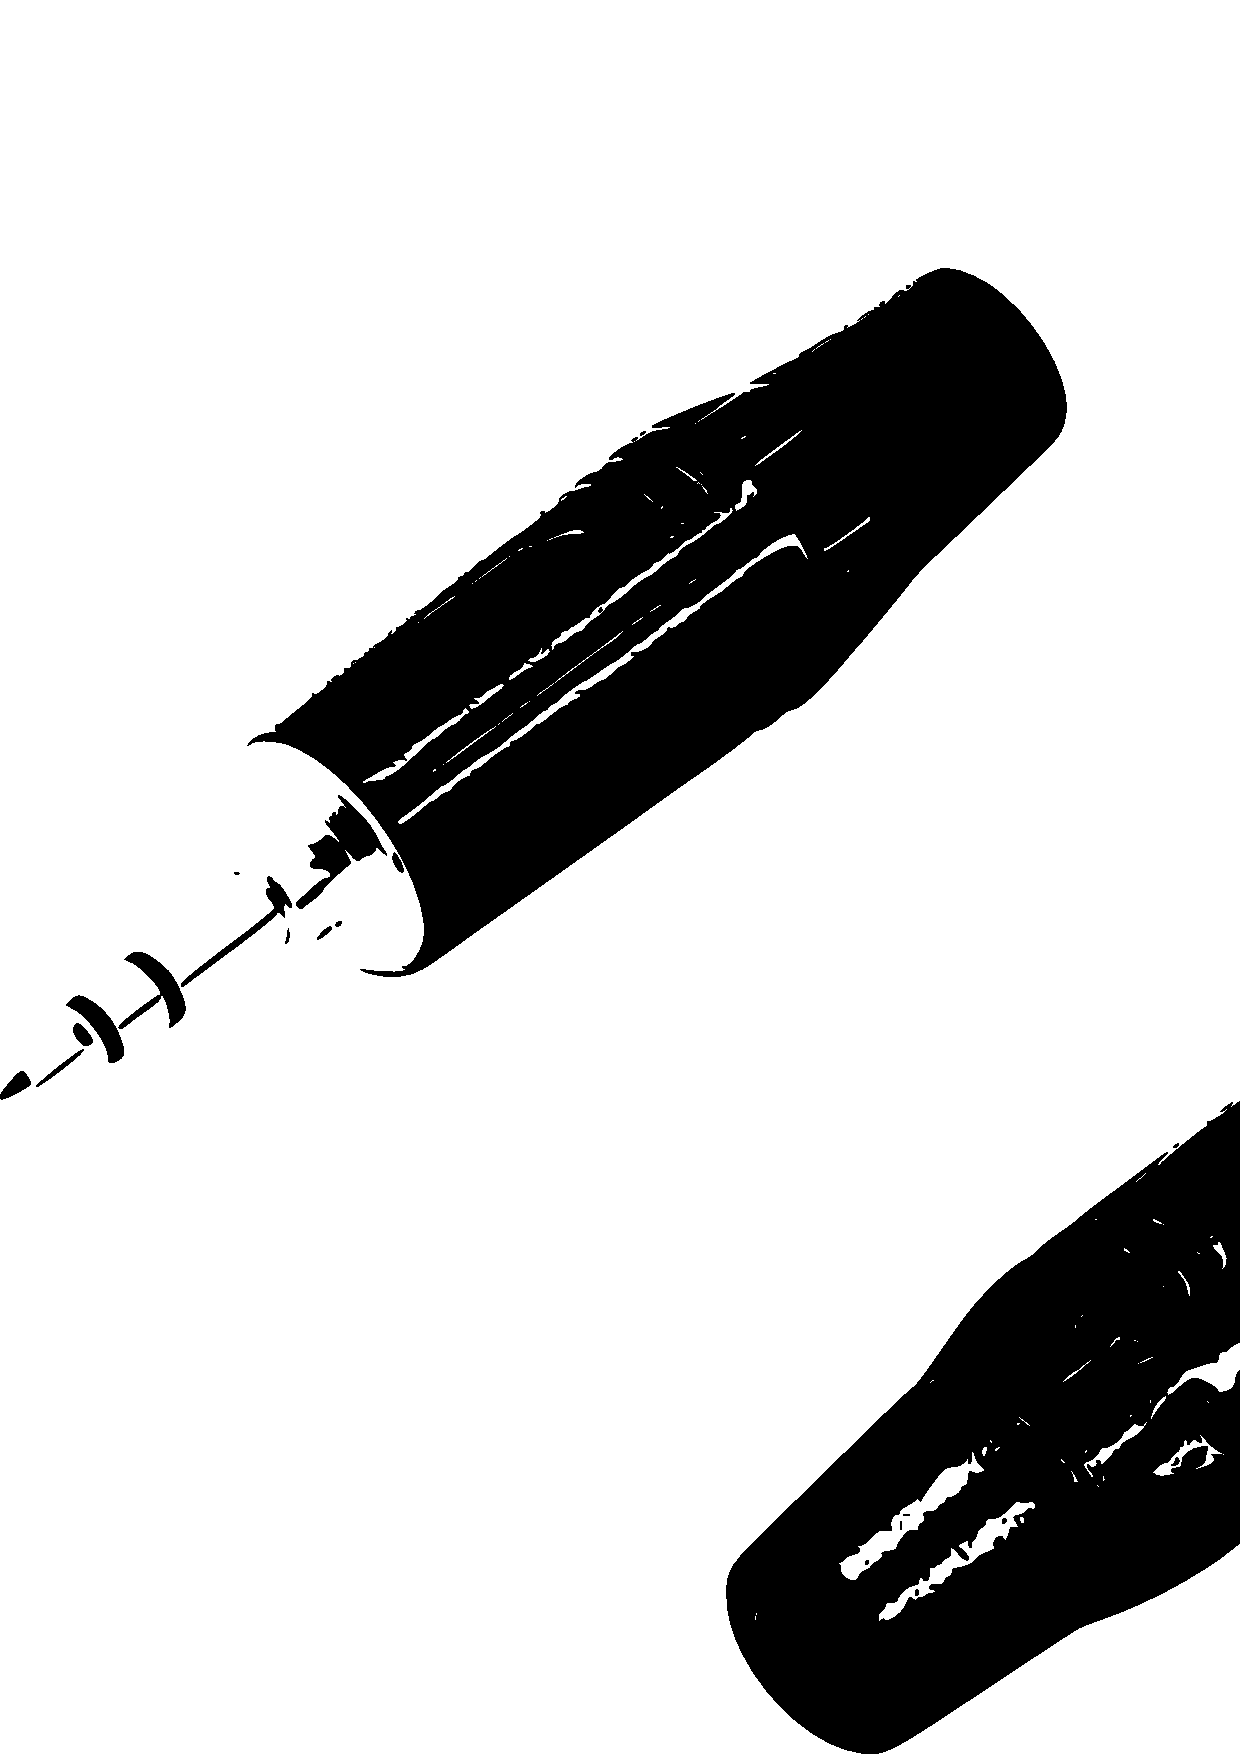
\includegraphics[scale=0.2]{figuras/fig20.png}
	\caption{plug 1/8$"$}
	\label{fig20}
\end{figure}

Outra versão existente é o conector de 2.5 mm, que muitas vezes, ao invés de dois fios para o transmissão de sinais, conta com três; muitas vezes para adicionar o microfone em \textit{headsets}. Esse conector pode ser visto na Figura \ref{fig21}.

\begin{figure}[h]
	\centering
    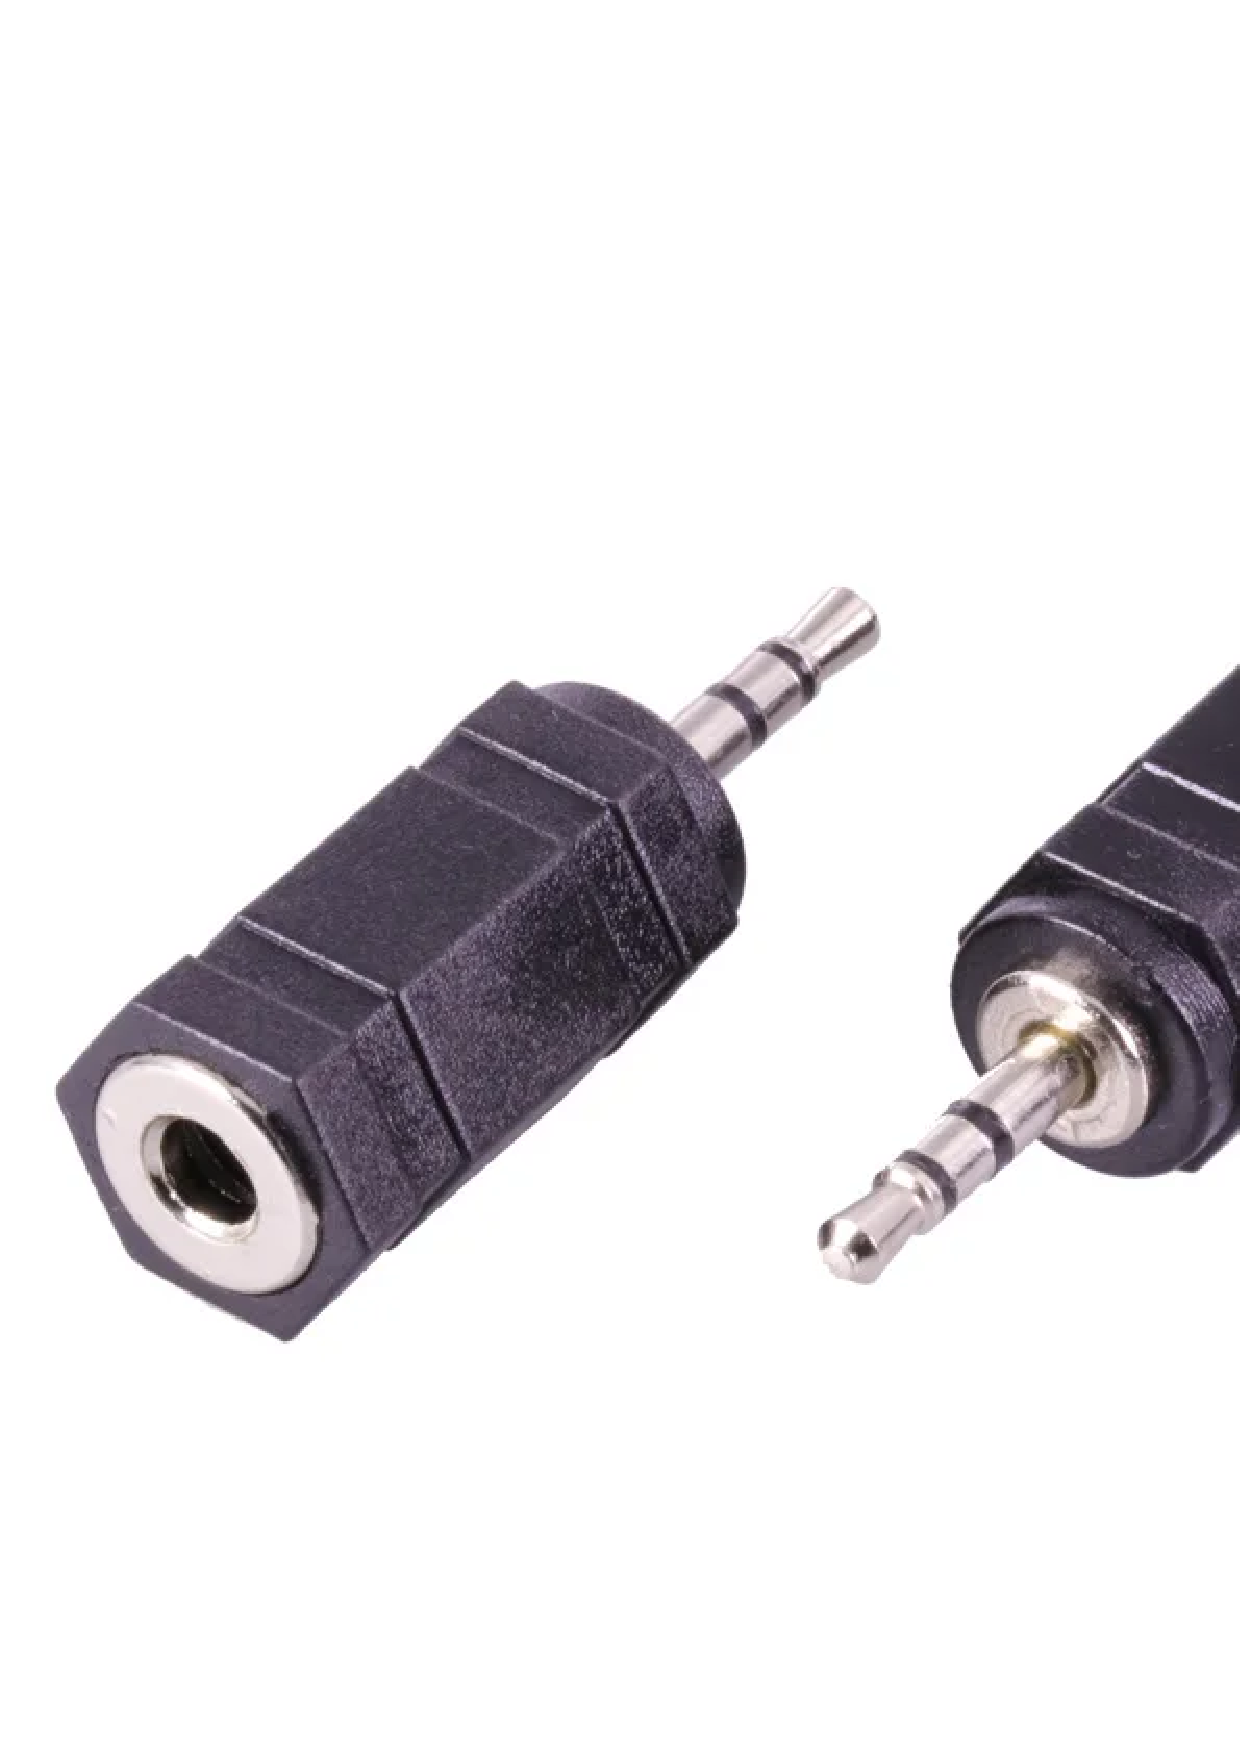
\includegraphics[scale=0.2]{figuras/fig21.png}
	\caption{plug 2,5 mm}
	\label{fig21}
\end{figure}

\subsection{RCA}
 O cabo RCA, Figura \ref{fig22}, muito utilizado nos primórdios de sistemas de telefonia, são também chamados de \textit{phono} devido ao seu uso em toca discos fonográficos. Cada cabo RCA tem a capacidade de transmitir, de forma não-balanceada, sinais de áudio mono. Dessa forma, caso se queira transmitir um sinal de som estéreo, utiliza-se dois cabos RCA. Caso conecte-se um som mono, internamente há um chaveamento capaz de transmitir o sinal que tem apenas uma entrada, mono, e retransmiti-la pelo outro canal, de forma que os dois canais transmitam o mesmo sinal de áudio \cite{bartlett}.

 \begin{figure}[h]
	\centering
    \includegraphics[scale=0.1]{figuras/fig22.png}
	\caption{cabo RCA}
	\label{fig22}
\end{figure}

\subsection{XLR}
É um tipo de conector de baixa voltagem chamado inicialmente de Cannon. Ele foi criado pela empresa Cannon com o intuito de transmissão de sinais balanceados para aplicações profissionais devido a sua rejeição de ruídos e pela integridade do sinal \cite{bartlett}. Esse conector pode ser visto na Figura \ref{fig23}.

\begin{figure}[h]
	\centering
    \includegraphics[scale=0.2]{figuras/fig23.png}
	\caption{cabo XLR}
	\label{fig23}
\end{figure}

\subsection{Protocolos Digitais}

Conectores para transmissão de dados digitais também são utilizados em \textit{mixers} e inúmeros outros equipamentos relacionados a áudio. Conectores como \textit{Ethernet} e \textit{Switch}, USB, \textit{bluetooth} e MIDI também são utilizados para diversas configurações de equipamentos.
  
\subsection{Amplificação de Potência}

Os principais níveis de tensões e potência existentes que mais são conectados a \textit{mixers} são o \textit{Phono} e nível de linha. A tensão do \textit{Phono} se encontra entre 0,1 a 5 mV e a tensão de um nível de linha se encontra em torno de 2,0 $V_{RMS}$. Segundo \cite{self2013audio}, é necessário que haja um intervalo de níveis de tensão para que o sinal possua um bom comportamento dentro do amplificado, de forma que não seja baixo o suficiente para que os ruídos sejam maiores e se tornem mais presentes do que os próprios sinais, nem altos suficiente para que sejam saturados após a amplificação. 
\par
Dessa forma, quando um sinal \textit{phono} entra no \textit{mixer}, ele precisa ser amplificado internamente.

\subsection{Equalização}

Conforme visto em seções anteriores, pode-se dividir todas as sub-bandas de frequência de som audível em três grande bandas: agudos, médios e graves. 
\par
Dessa forma, tradicionalmente, após o sinal ser amplificado, dentro do \textit{mixer} pode haver controle de ganho ou atenuação das bandas.
\par
À medida que a mixagem acontece, determinadas combinações de uso do ganho podem ser acionados. E, num estágio posterior, todos os canais são somados.

\subsection{\textit{Trim} e Volume}
Quanto à amplitude do sinal de áudio, há dois controles que frequentemente estão presentes em \textit{mixers}: \textit{trim} e volume. O \textit{trim} é um controle sobre o ganho que um sinal obtém antes de ser processado pelo \textit{mixer} e passar pelos controles de equalização. Serve para que o usuário consiga ajustar dois tipos de sinais para que apresentem o mesmo nível ou a combinação desejada; uma mais presente que a outra.
\par
Já o volume é geralmente visto em um controle de \textit{fader}. Esse botão serve para controlar a amplitude do sinal enquanto o sinal é equalizado, ou seja, posteriormente à amplificação do sinal.

\subsection{Conversão AD/DA}
Quanto ao processamento dos sinais de áudio, pode-se dividir o tipo de processamento em dois grandes bloco: analógicos e digitais. Analógicos são feitos por circuitos analógicos e digitais são por computadores, DSPs e outros dispositivos. Porém, a diferença primordial é o estado no qual o sinal, enquanto processado, se encontra. Caso o sinal, enquanto esteja sendo processado, for analógico, o mixer é analógico, e vice-versa.
\par
Dispositivos que reproduzem música como CDJs e toca-discos podem emitir sinais analógicos ou digitais, dependendo do equipamento e da saída utilizada. 
Dessa forma, caso o \textit{mixer} necessite de sinais digitais e a saída do reprodutor de música for analógico, deve-se realizar a conversão analógico digital e vice-versa.
\par
De forma parecida, o sinal de saída do \textit{mixer} deve ser analógica pois passará por um amplificador de potência para que, posteriormente, vá para alto-falantes. Ou seja, caso o processamento seja realizado de forma digital, o sinal deve passar por uma conversão digital analógica.




%\subsection{PureData}
%Dentro dos sinais digitais, há inúmeras formas de se processar sinais. Pode-se usar diversas linguagens de programação como PureData, MAX, SuperCollider, CSound, Faust e Chuck que são dedicadas a processamento de áudio. Já há outras linguagens de finalidades diversas como JavaScript, C, C++, Rust e outros que também contam com aplicações a áudio.
%\par
%Cada linguagem possui sua especificidade, vantagens, desvantagens, aplicações e suportes. Por isso, a escolha da linguagem deve levar em conta as especificações dos requisitos que o projeto demanda.
%\par


